\subsection{Interface} % (Jan Pieter)

% include common command to define the windows.
% Define some common stuff to draw circuits. The commands defined can be
% used in a draw command, i.e.:
% \draw (x, y) \gateAND -- ++( 1, 0) \gateNOT ++( 1, 0) \terminal;
\tikzstyle{terminal}=[circle,fill=black,inner sep=1.5pt]
\newcommand{\terminal}{node[terminal]{}}

% define a wire command. out= ++(2, 0)
\newcommand{\wire}{\terminal -- ++( 2, 0) }

% define a AND gate with start coord first in-terminal, coords from in1:
% in2= ++(0, -.6)
% out= ++(2, -.3)
\newcommand{\gateAND}{
	\terminal -- ++(.5, 0) -- ++(0,-0.6) -- ++(-.5, 0) \terminal -- ++(.5, 0) -- ++(0, -.2) [rounded corners=15pt] --  ++(1, 0)  -- ++(0, 1) [sharp corners] -- ++(-1, 0) -- ++(0, -.2)  ++(1, -0.3) -- ++(0.5, 0)
}

% define a NOT gate with start coord on in-terminal, coord from in:
% out= ++(2, 0)
\newcommand{\gateNOT}{
	\terminal -- ++(.5, 0) --  ++(0, .5) -- ++(1, -.5) -- ++(-1, -.5) -- ++(0, .5) ++(1, 0) -- ++(0.5, 0)
}

\newcommand{\programGUI}[1]{
	\draw[fill=black!20,line width=1] (-6,4) rectangle ++(12, -7.5);

	% window title bar
	\draw[fill=black!15,line width=1] (-6,4) rectangle (6, 3.5);
	\node[draw, anchor=north west] at (-6, 4) {Brick};
	\node[draw, anchor=north west] at (-4.8, 4) {Simulate};
	\node [anchor=north] at (0, 4) {Synthbio - #1}; %file title
	\node [anchor=east] at (6, 3.75) {\_ [] X}; % minimize maximize close

}
\newcommand{\sidebar}{
	% sidebar
	\draw[fill=black!20,line width=1] (-6, 3.5) rectangle ++(3, -3.5) rectangle ++(-3, -3.5);
	\draw (-5.5, 3) \wire \terminal;
	\draw (-5.5, 2.5) \gateAND \terminal;
	\draw (-5.5, 1) \gateNOT \terminal;{}

	\node[anchor=north west] at( -6, 0) {\tiny User defined bricks};
}


When starting the program for the first time, the user is presented with window in build mode (figure~\ref{fig-interface-empty}) containing a sidebar with the three elemental building blocks: wire, an AND-gate and a NOT-gate. The lower part of the sidebar is reserved for user-defined \textit{substructures}, as mentioned in functional requirement 1.
The remainder of the window is a working area which is initially empty.
On the top bar two menu items are present. One for basic file actions like export, save and import, the second for actions concerning the simulation of the brick.

\begin{figure}[h!]
	\caption{Initial program state.}
	\label{fig-interface-empty}
	\centering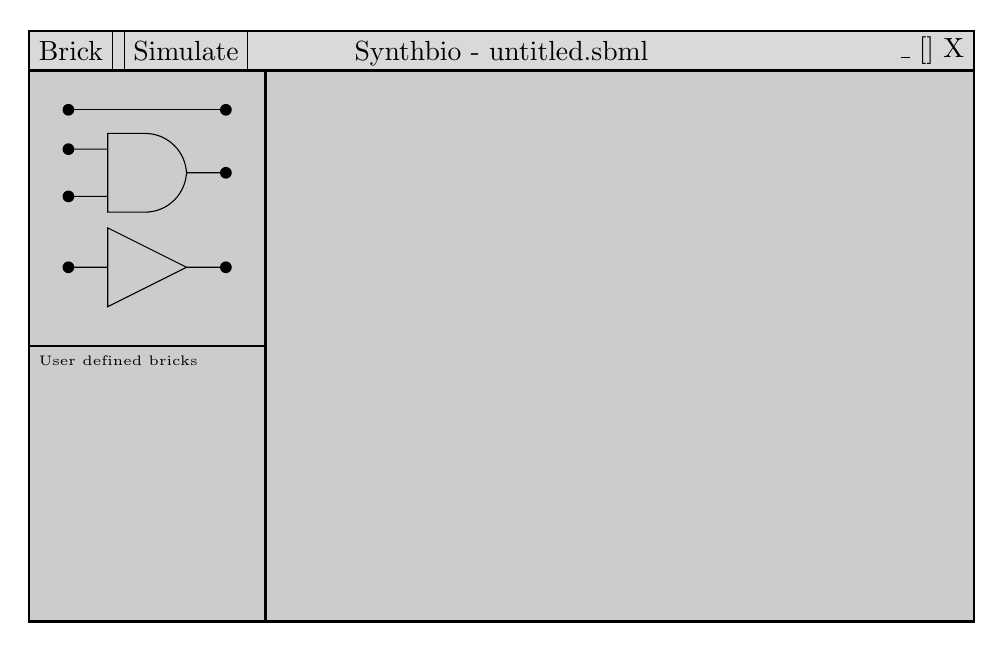
\begin{tikzpicture}
		\programGUI{untitled.sbml}
		\sidebar
	\end{tikzpicture}
\end{figure}

\noindent To model a circuit, the elemental parts can be dragged into the working area, the gates may be connected using wires. The interface state after adding some wires is proposed in figure~\ref{fig-interface-building}.

\begin{figure}[h!]
	\caption{After adding some gates to the working area.}
	\label{fig-interface-building}
	\centering
	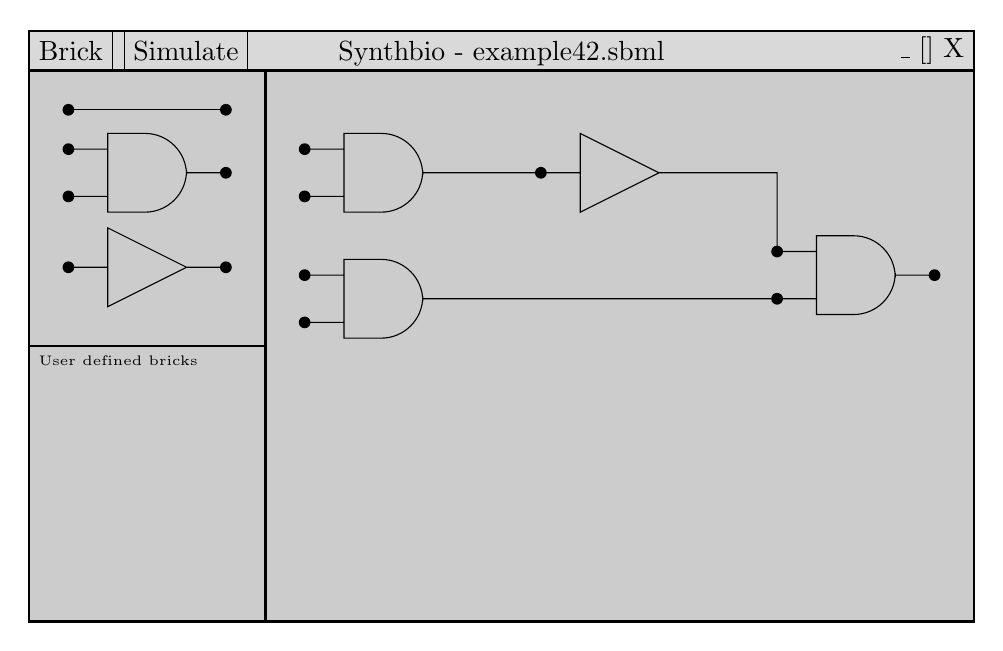
\begin{tikzpicture}
		\programGUI{example42.sbml}
		\sidebar

		%define some gates in working area
		\draw ( -2.5, 2.5) \gateAND -- ++(1, 0) \gateNOT -- ++(1, 0) -- ++(0, -1) \gateAND \terminal;

		\draw ( -2.5, .9)  \gateAND -- ++( 4,0);
		
	\end{tikzpicture}
\end{figure}

\pagebreak
\noindent After building the circuit, the user has to select which protein to use for each signal. This can be done during the building process aswell. In figure~\ref{fig-interface-selectProtein} the protein selection dialog is shown for one signal, for some other signals the representing protein is shown above.
\begin{figure}[h!]
	\caption{Selecting a protein for the signal.}
	\label{fig-interface-selectProtein}
	\centering
	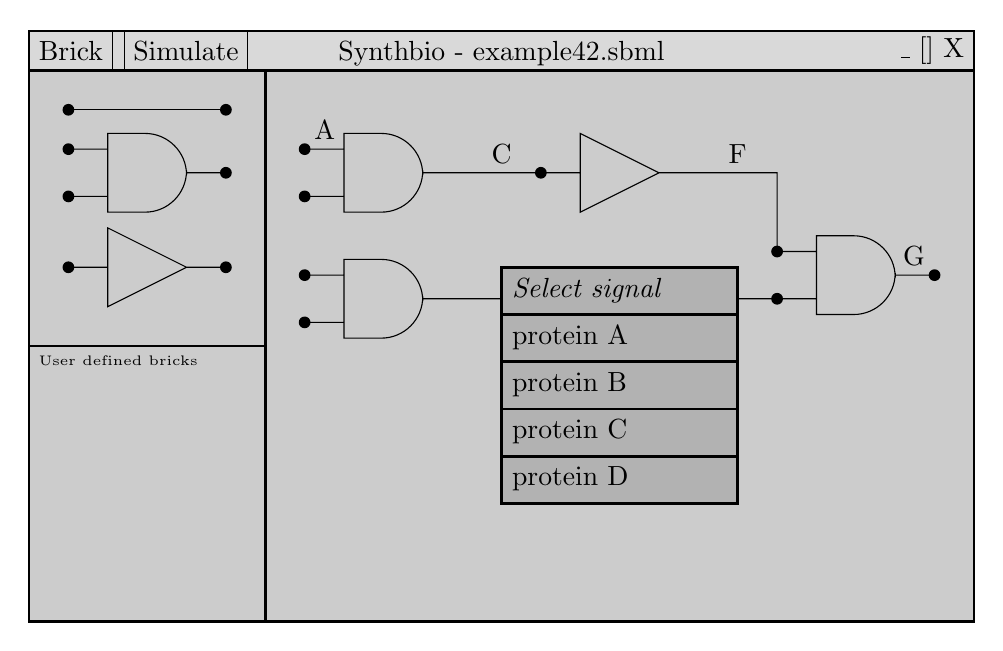
\begin{tikzpicture}
		\programGUI{example42.sbml}
		\sidebar

		\draw ( -2.5, 2.5) node[above right] {A} \gateAND -- node [above] {C} ++(1, 0) \gateNOT -- node [above] {F} ++(1, 0) -- ++(0, -1) \gateAND node[above left] {G} \terminal ;
	
		\draw ( -2.5, .9)  \gateAND -- ++( 4,0);

		\draw ( 0, 1) [fill=black!30,line width=1pt] rectangle ++(3, -3)
			++(-3, 3) node [anchor=north west] {\textit{Select signal}} rectangle ++(3, -.6)
			++(-3, 0) node [anchor=north west] {protein A} rectangle ++(3, -.6)
			++(-3, 0) node [anchor=north west] {protein B} rectangle ++(3, -.6)
			++(-3, 0) node [anchor=north west] {protein C} rectangle ++(3, -.6)
			++(-3, 0) node [anchor=north west] {protein D} rectangle ++(3, -.6);
	\end{tikzpicture}
\end{figure}


\noindent If the user is satisfied with the circuit, the simulate mode can be selected. For each input protein, the concentration as a function of time can be changed. The program will calculate and display the results as shown in figure~\ref{fig-interface-simulation}.
\begin{figure}[h!]
	\caption{Simulation of the BioBrick}
	\label{fig-interface-simulation}
	\centering\begin{tikzpicture}
		\programGUI{simulate.sbml}

		% circuit
		\draw ( -4.5, 3) node[above right] {A} \gateAND -- node [above] {E} ++(1, 0) \gateNOT -- node [above] {F} ++(1, 0) -- ++(0, -1) \gateAND node[above left] {G} \terminal ;
		\draw ( -4.5, 1.4) node[above right] {C} \gateAND -- node [above] {H} ++( 4,0);
		\node [above right] at(-4.5, 2.4) {B};
		\node [above right] at(-4.5, .8) {D};

		%simulation
		\draw (-6, 0 ) -- +(12, 0);
		\node[anchor=north west] at (-6, 0) {Inputs};
		\node[anchor=north west] at (-6, -1.6) {Outputs};

		\newcommand{\dt}{.2}
		%~ % n \dt-steps forward
		\newcommand{\fw}{ ++(\dt, 0)}
		% random step forward
		\newcommand{\randfw}{ ++(\dt+rnd*8*\dt, 0)}
		
		\newcommand{\up}{ ++(0, \dt)}
		\newcommand{\down}{ ++(0, -\dt)}
		\newcommand{\randOn}{\up -- \randfw -- \down}
		
		\newcommand{\signal}{\randfw -- \randOn -- \fw -- \randOn -- \randfw -- \randOn -- \randfw -- \randOn -- \fw -- \randOn}

		\newcommand{\y}{.1-\n*0.4}
		\foreach \name [count=\n] in {A, B, ..., H}{
			\draw[dotted] (-4, \y) -- ++(10, 0);
			\draw (-4.4, \y) node {\name} ++(.5, 0) -- \signal -- ( 6, \y);
		}
	\end{tikzpicture}
\end{figure}
